\chapter{Extended Results}
\label{app:extended}

This appendix collects the hyperparameter configurations, supplementary figures, and environment details that scale and reproduce the results of Chapter~\ref{chap:results}. The material here is referenced from the main text where it supports a specific claim; none of the numbers reported in Chapters~\ref{chap:results}--\ref{chap:conclusion} depend on reading this appendix.

\section{Hyperparameter configurations}
\label{app:hyperparameters}

Table~\ref{tab:app_hyperparams_networks} lists the final hyperparameters for every trained inverse-kinematics or forward-kinematics network reported in Chapter~\ref{chap:results}. Architecture widths, optimiser, learning rate, batch size, epoch cap, early-stopping patience, random seed, and the best-epoch indices returned by the early-stopping monitor are shown. All values are those fixed after the preliminary sweeps described in Section~\ref{sec:hyperparam}; they are identical across both datasets unless the $n_{p}$-dependent output width is indicated.

\begin{table}[!htbp]
  \centering
  \footnotesize
  \setlength{\tabcolsep}{4pt}
  \caption{Final hyperparameter configurations for every trained network, matched to the registered YAML configurations in \texttt{configs/*.yaml}. Output width equals $n_{p}$ for inverse-kinematics networks and $3$ for forward-kinematics networks. MLP architectures are reported as input--hidden$_{1}$--hidden$_{2}$--hidden$_{3}$--hidden$_{4}$--output (four hidden layers throughout); LSTM architectures are reported as (window $W$, hidden units, layers). All networks use ReLU (MLP) or default PyTorch tanh/sigmoid (LSTM) activations, the Adam optimiser, and seed $42$. Input features are $(x,y,z)$ for tip-only IK networks, $(x,y,z,x_{m},y_{m},z_{m})$ for tip-plus-mid IK networks, and the pressure/valve command vector for FK arbiters.}
  \label{tab:app_hyperparams_networks}
  \begin{tabularx}{\linewidth}{@{}l l X l l l l@{}}
    \toprule
    Role & Dataset & Architecture & Lr & Batch & Cap / pat. & Best ep. \\
    \midrule
    IK MLP tip-only         & Dataset 1 & 3--128--256--256--128--6  & $10^{-3}$ & 64 & 500 / 30 & 4   \\
    IK MLP tip-plus-mid     & Dataset 1 & 6--128--256--256--128--6  & $10^{-3}$ & 64 & 500 / 30 & 21  \\
    IK MLP tip-only         & Dataset 2 & 3--64--128--128--64--3    & $10^{-3}$ & 64 & 500 / 30 & 44  \\
    IK LSTM tip-only        & Dataset 1 & ($W{=}10$, $128$, $2$)    & $10^{-3}$ & 64 & 300 / 20 & 38  \\
    IK LSTM tip-plus-mid    & Dataset 1 & ($W{=}10$, $128$, $2$)    & $10^{-3}$ & 64 & 300 / 20 & 45  \\
    IK LSTM tip-only        & Dataset 2 & ($W{=}10$, $128$, $2$)    & $10^{-3}$ & 64 & 300 / 20 & 114 \\
    FK arbiter              & Dataset 1 & 6--128--256--256--128--3  & $10^{-3}$ & 64 & 500 / 30 & 82  \\
    FK arbiter              & Dataset 2 & 3--64--128--128--64--3    & $10^{-3}$ & 64 & 500 / 30 & 156 \\
    Sim2Real Strategy A     & Dataset 2 & 3--64--128--128--64--3    & $10^{-3}$ & 64 & 500 / 30 & 137 \\
    Sim2Real B (pre-train)  & synthetic & 3--64--128--128--64--3    & $10^{-3}$ & 64 & 100 / --- & --- \\
    Sim2Real B (fine-tune)  & Dataset 2 & 3--64--128--128--64--3    & $10^{-4}$ & 64 & 500 / 30 & 71  \\
    Sim2Real Strategy C     & synthetic & 3--64--128--128--64--3    & $10^{-3}$ & 64 & 500 / 30 & 198 \\
    \bottomrule
  \end{tabularx}

  \vspace{0.5em}
  \noindent\emph{Note.} Strategy~B's pre-training phase runs for a fixed cap of $100$ epochs with no early-stopping monitor, so no best-epoch index is reported for that phase; both phases of Strategy~B share the same network architecture and scalers, which are fitted on the real subset so the synthetic pre-training data is transformed into the target-domain standardisation (Section~\ref{sec:sim_transfer}). The Dataset~2 MLP best-epoch of $44$ matches the training-curve dotted marker of Figure~\ref{fig:app_training_curves}; the FK arbiter and Dataset~2 LSTM values are read from their respective training runs on the same configuration.
\end{table}

Table~\ref{tab:app_hyperparams_solvers} collects the hyperparameters of the non-learned components: the SLSQP two-segment PCC inverse of Section~\ref{sec:pcc_multi} and the damped-least-squares Jacobian iteration of Section~\ref{sec:jacobian}. These values were fixed in advance from the referenced literature and are reported here for completeness.

\begin{table}[!htbp]
  \centering
  \small
  \caption{Hyperparameters of the optimisation-based and iterative solvers.}
  \label{tab:app_hyperparams_solvers}
  \begin{tabularx}{\linewidth}{@{}l l X@{}}
    \toprule
    Component & Parameter & Value \\
    \midrule
    \multirow{4}{*}{Two-segment PCC SLSQP} & Bounds $\theta_{s}$            & $[0,\, 2.5]$\,rad per segment \\
                                            & Bounds $\varphi_{s}$           & $[-\pi,\, \pi]$\,rad per segment \\
                                            & Bounds $\Delta L_{s}$          & $[-50,\, +50]$\,mm per segment \\
                                            & Termination tolerance          & $10^{-8}$ on objective gradient \\
    \midrule
    \multirow{6}{*}{Jacobian DLS iteration} & Damping $\lambda$              & $0.05$ \\
                                            & Step scale $\alpha$            & $0.5$ \\
                                            & Position tolerance             & $1$\,mm \\
                                            & Max iterations                 & $50$ \\
                                            & Jacobian mode                  & PyTorch autograd on FK net \\
                                            & Initialisation                 & cold (mid-range) \textit{or} warm (MLP prediction) \\
    \bottomrule
  \end{tabularx}
\end{table}

\section{Exploratory data analysis: protocol}
\label{app:eda_protocol}

Each dataset was examined before model training to verify raw-data format, validate the preprocessing assumptions of Section~\ref{sec:splits}, and (for Dataset~1) estimate the physical noise floor.

\paragraph{Dataset~1 checks.}
(i) Per-recording spatial standard deviation of the base-marker mean position, as a base-stationarity check within each recording. (ii) Overlaid four-seed base-relative tip point clouds, as a check for rotational drift between recording sessions. (iii) Seed-0 repeatability from the three repeated trials: each tip sample in one trial was paired with its nearest neighbour in the other two trials in the six-dimensional pressure-command space, and the standard deviation of the three paired tip positions was recorded per frame. Nearest-neighbour matching was preferred over index alignment because the seed-0 command sequences differed slightly across trials; see Appendix~\ref{app:eda_detail}.

\paragraph{Dataset~2 checks.}
(i) Missing-value and duplicate-row counts. (ii) Per-column histograms for truncation, clipping, or quantisation artefacts. (iii) A shuffled-vs-ordered step-size ratio to test whether consecutive rows carry any temporal dependency: the mean Euclidean step between consecutive rows was compared against the analogous statistic under row permutation, in both tip-position space and valve-command space. (iv) Pearson correlations between each valve command and each tip coordinate as a non-degeneracy sanity check on the actuation--pose map.

\section{Exploratory data analysis: findings in detail}
\label{app:eda_detail}

\paragraph{Dataset~1 occlusion.}
All six recordings contain exactly $4{,}000$ raw frames ($24{,}000$ total). Marker drop-outs lost $64$ frames in aggregate ($0.27\%$), distributed unevenly across recordings (Table~\ref{tab:app_eda_ds1_occlusion}). The mid and tip triad occlusion masks were identical per recording, so the same $23{,}936$ frames remain usable for both the tip-only and the tip-plus-mid variants.

\begin{table}[!htbp]
  \centering
  \small
  \caption[Per-recording occlusion counts for Dataset~1.]{Per-recording occlusion counts for Dataset~1. Each recording contains $4{,}000$ raw frames; usable frames are those in which every marker in the mid and tip triads was visible.}
  \label{tab:app_eda_ds1_occlusion}
  \begin{tabularx}{\linewidth}{@{}l l X X X@{}}
    \toprule
    Seed & Trial & Raw frames & Usable frames & Occlusion \\
    \midrule
    1 & 1 & $4{,}000$ & $3{,}981$ & $0.48\%$ \\
    2 & 1 & $4{,}000$ & $4{,}000$ & $0.00\%$ \\
    3 & 1 & $4{,}000$ & $3{,}999$ & $0.03\%$ \\
    0 & 1 & $4{,}000$ & $3{,}990$ & $0.25\%$ \\
    0 & 2 & $4{,}000$ & $4{,}000$ & $0.00\%$ \\
    0 & 3 & $4{,}000$ & $3{,}966$ & $0.85\%$ \\
    \bottomrule
  \end{tabularx}
\end{table}

\paragraph{Dataset~1 base stationarity.}
Five of six recordings showed apparent base motion of up to $\sim$$32$\,mm in the per-frame base-mean spatial standard deviation; inspection of the raw marker stream showed this was an NaN-aware-mean artefact (when one or two of the three base markers were momentarily occluded, the mean collapsed onto the remaining marker's cluster-centroid offset). Once occluded frames were removed, the standard deviation fell below optical marker resolution, so the base is treated as fixed within every recording and the translation-only preprocessing of Section~\ref{sec:splits} is justified.

\paragraph{Dataset~1 tip and mid magnitudes.}
Mean base-relative tip magnitude $\approx 375$\,mm (max $\approx 405$\,mm, consistent with the $\sim$$410$\,mm assembled length); mean mid magnitude $\approx 198$\,mm, consistent with the mid-section sitting near the arm midpoint. Both fall within the $500$\,mm sanity threshold of the loader.

\paragraph{Dataset~1 seed-0 repeatability distribution.}
The paired per-frame tip standard deviation across the three seed-0 trials has mean $2.29$\,mm, median $1.88$\,mm, and $95$th percentile $4.14$\,mm, with a long tail to $60.3$\,mm driven by isolated frames near occlusion gaps (Fig~\ref{fig:app_ds1_repeatability}). The $\sim$$2.3$\,mm mean is cited as the Dataset~1 physical noise floor in Section~\ref{sec:eda_findings} and subsequent chapters.

\begin{figure}[!htbp]
  \centering
  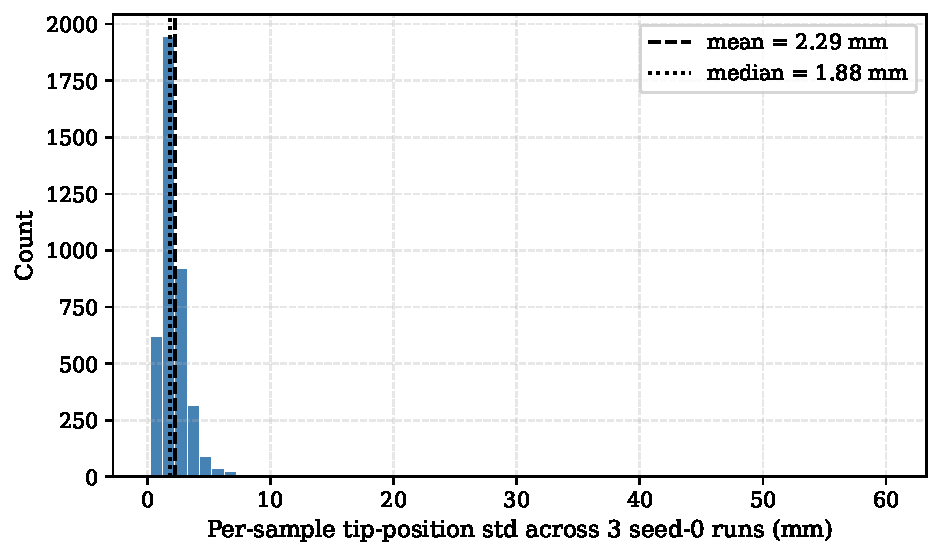
\includegraphics[width=0.75\linewidth]{fig/ds1_seed0_repeatability.pdf}
  \caption[Seed-0 repeatability distribution for Dataset~1.]{Per-sample tip-position standard deviation across the three repetitions of the Dataset~1 seed-0 recording, with frames paired by nearest neighbour in the six-dimensional pressure-command space.}
  \label{fig:app_ds1_repeatability}
\end{figure}

\paragraph{Dataset~1 seed-0 command non-identity.}
Contrary to the expectation set by a shared RNG seed, the three seed-0 pressure-command sequences were not bit-identical: mean per-frame Euclidean distance between repetition 1 and 2 was $13.2$ raw units, between 1 and 3 was $45.2$ raw units (range $[0, 100]$). Index-aligned pairing would therefore compare slightly different commands, which is why the nearest-neighbour matching above was adopted.

\paragraph{Dataset~2 integrity.}
$18{,}072$ rows, no missing values, no duplicate rows. Valve commands integer-valued in $[0, 2500]$; every row inside this band. After inch-to-millimetre conversion the tip coordinates span $[-47.9, 53.8]$\,mm ($X$), $[-47.7, 56.1]$\,mm ($Y$), $[-27.5, 36.9]$\,mm ($Z$).

\paragraph{Dataset~2 temporal structure (absent).}
Mean Euclidean consecutive-row step in tip-position space $32.49$\,mm, versus $33.84$\,mm under row permutation (ratio $0.96$). The same statistic in three-dimensional valve-command space gives ratio $1.003$. Both ratios are indistinguishable from unity, so the rows of Dataset~2 behave as IID samples rather than as a trajectory. The default $70/15/15$ order-preserving split of Section~\ref{sec:splits} was retained as a precaution against subtle residual structure.

\paragraph{Dataset~2 actuation--pose correlation.}
Every valve--coordinate Pearson coefficient has magnitude above $0.09$ (Fig~\ref{fig:app_ds2_correlation}); the strongest entries are consistent with three chambers at $120^{\circ}$ (valve~1: $-Y, +Z$; valve~2: $+X$; valve~3: $-X$). The actuation--pose map is non-degenerate.

\begin{figure}[!htbp]
  \centering
  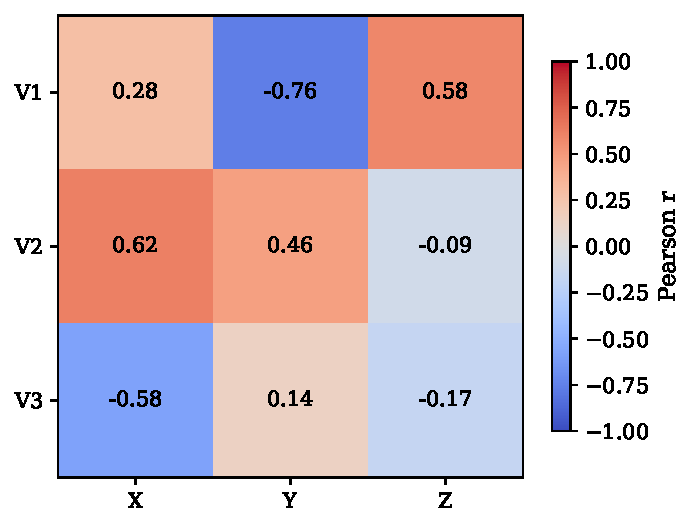
\includegraphics[width=0.6\linewidth]{fig/ds2_correlation.pdf}
  \caption[Actuation--pose correlation matrix for Dataset~2.]{Pearson correlation between each valve command and each tip coordinate across the $18{,}072$ rows of Dataset~2. The strongest per-row entries are consistent with a three-chamber radial actuator at $120^{\circ}$.}
  \label{fig:app_ds2_correlation}
\end{figure}

\section{Supplementary figures}
\label{app:extended_figures}

Figure~\ref{fig:app_training_curves} shows the training and validation loss curves for the feed-forward networks of Section~\ref{sec:res_mlp_tip} on both datasets. The Dataset~1 curve flattens around epoch $4$ and the validation loss starts to increase thereafter, so early stopping selects the fourth-epoch checkpoint and confirms the data-limited plateau discussed in Section~\ref{sec:disc_jacobian_vs_mlp}. The Dataset~2 curve continues to descend for several tens of epochs before levelling off, with the validation-loss minimum at epoch~$44$; this is consistent with the single-valued inverse being learnable from the available sample count.

\begin{figure}[!htbp]
  \centering
  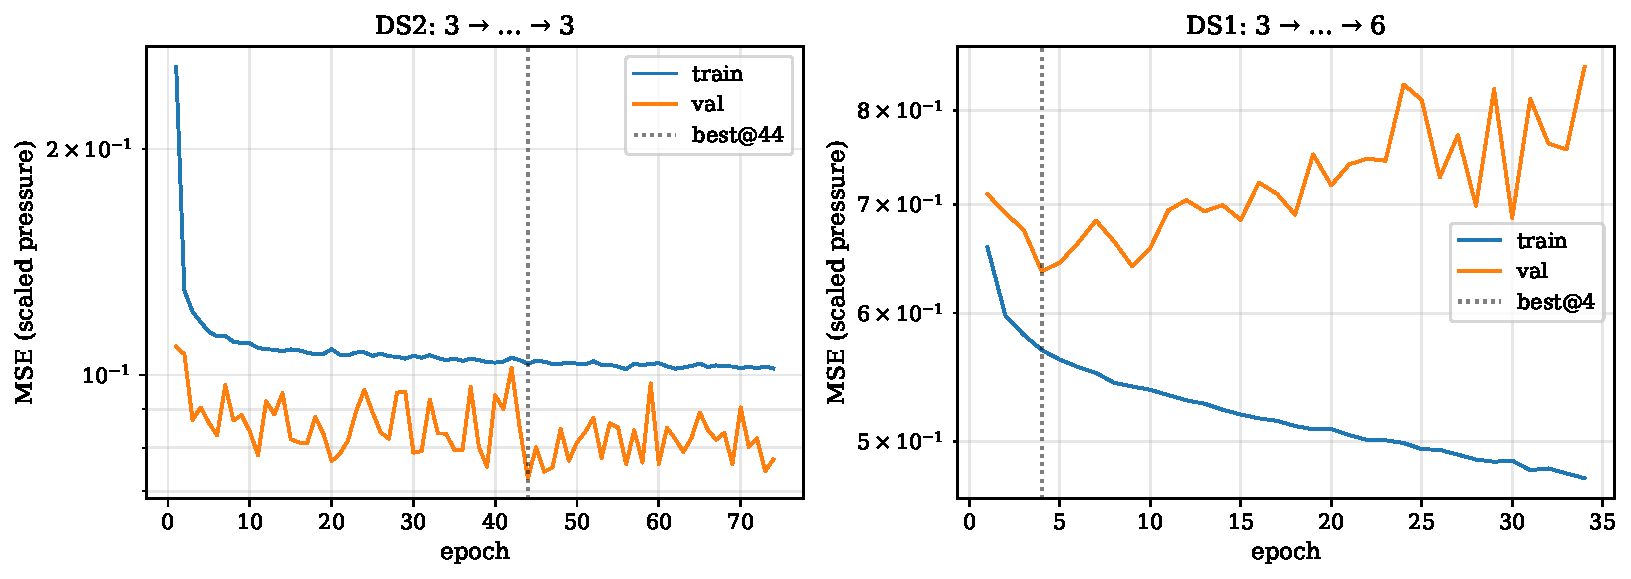
\includegraphics[width=0.92\linewidth]{fig/mlp_training_curves.pdf}
  \caption[Training and validation loss of the tip-only MLPs.]{Training and validation loss as a function of epoch for the tip-only MLP on Dataset~2 (left) and Dataset~1 (right). The vertical axis is mean squared error on the $z$-score-standardised pressure targets (not raw-unit MAE), the loss function actually optimised during training; raw-unit MAE is reported in the main results tables. Vertical dotted lines mark the early-stopping best-epoch indices ($44$ for Dataset~2, $4$ for Dataset~1), which are the indices recorded in Table~\ref{tab:app_hyperparams_networks}.}
  \label{fig:app_training_curves}
\end{figure}

Figure~\ref{fig:app_mlp_sweep} presents the hyperparameter sweep heatmap referenced in Section~\ref{sec:hyperparam}. Each cell reports the validation pressure MAE at the corresponding $(\text{hidden width}, \text{learning rate})$ combination on Dataset~2; the $128$-unit, $10^{-3}$ configuration chosen for all subsequent experiments is inside the region of flat near-optimal performance.

\begin{figure}[!htbp]
  \centering
  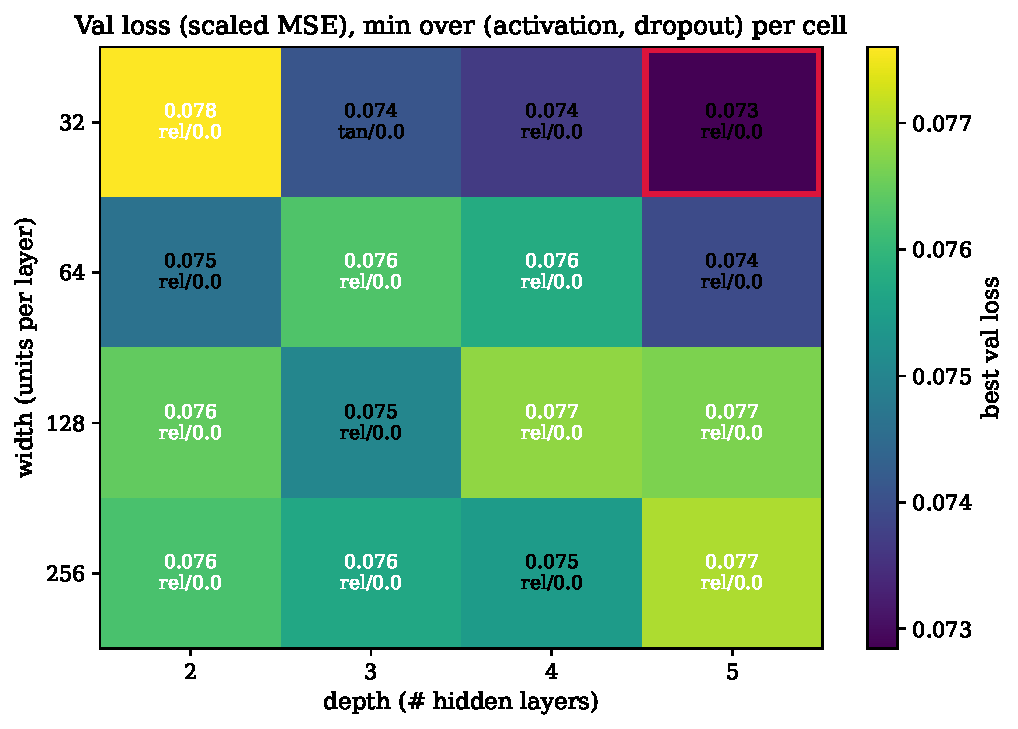
\includegraphics[width=0.78\linewidth]{fig/mlp_sweep_heatmap.pdf}
  \caption[Validation pressure MAE across the MLP hyperparameter sweep on Dataset~2.]{Validation pressure MAE across the MLP hyperparameter sweep on Dataset~2. Darker cells denote lower error. The configuration selected for all reported MLP experiments is marked with a white frame.}
  \label{fig:app_mlp_sweep}
\end{figure}

Figure~\ref{fig:app_jacobian_time} shows the per-target inference-time distribution of the warm-started Jacobian-learned iteration on both datasets, alongside the constant-cost feed-forward MLP baseline, as referenced in Section~\ref{sec:res_jacobian}. The Jacobian histogram is tightly peaked around $46$\,ms on both datasets, two to three orders of magnitude slower than the $\sim\!0.05$\,ms per-target MLP evaluation. The logarithmic horizontal axis makes the size of the latency gap visible at a glance.

\begin{figure}[!htbp]
  \centering
  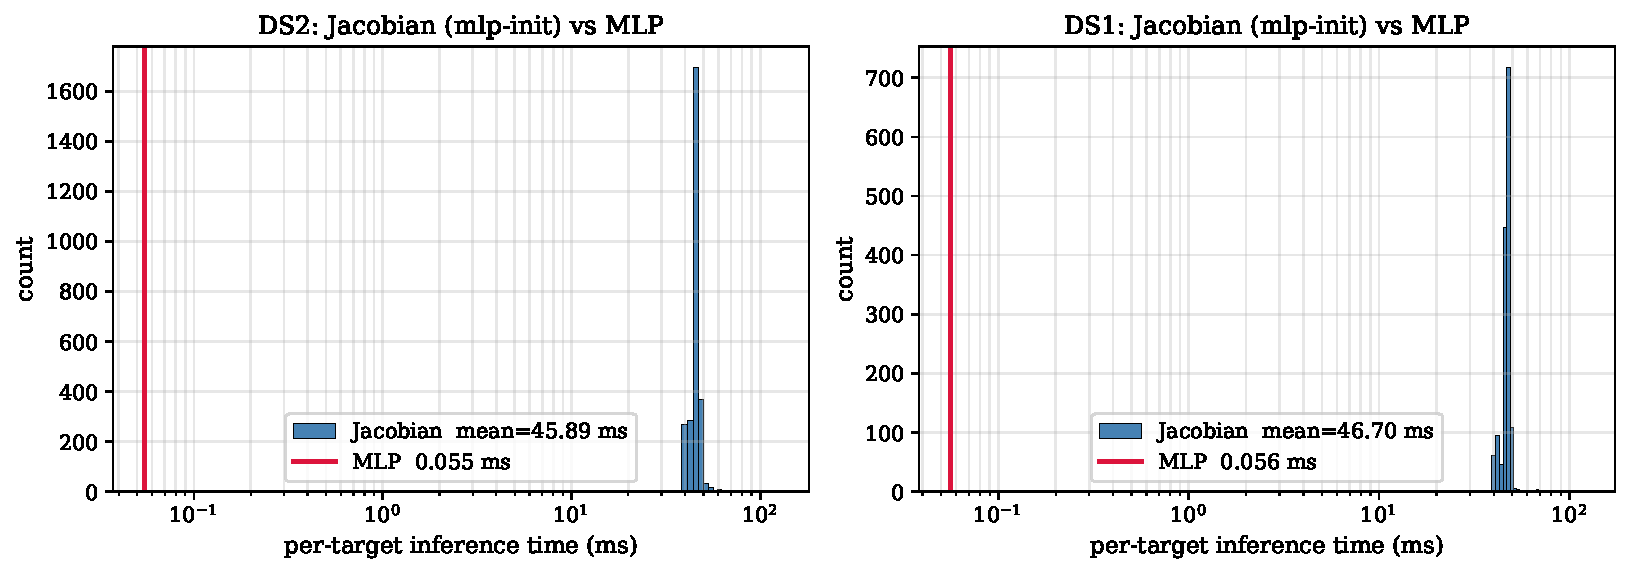
\includegraphics[width=0.95\linewidth]{fig/jacobian_inference_time.pdf}
  \caption[Per-target inference-time distributions: Jacobian-IK vs MLP.]{Distribution of per-target wall-clock inference time for the warm-started (MLP-initialised) Jacobian-learned iteration (blue histogram) and the feed-forward MLP baseline (red vertical line) on Dataset~2 (left) and Dataset~1 (right). The horizontal axis is logarithmic (milliseconds). Jacobian means are $45.89$\,ms on Dataset~2 and $46.70$\,ms on Dataset~1, against $0.055$\,ms and $0.056$\,ms for the MLP respectively; the Jacobian iteration is therefore roughly $830\times$ slower than the direct regressor on both platforms.}
  \label{fig:app_jacobian_time}
\end{figure}

\begin{figure}[!htbp]
  \centering
  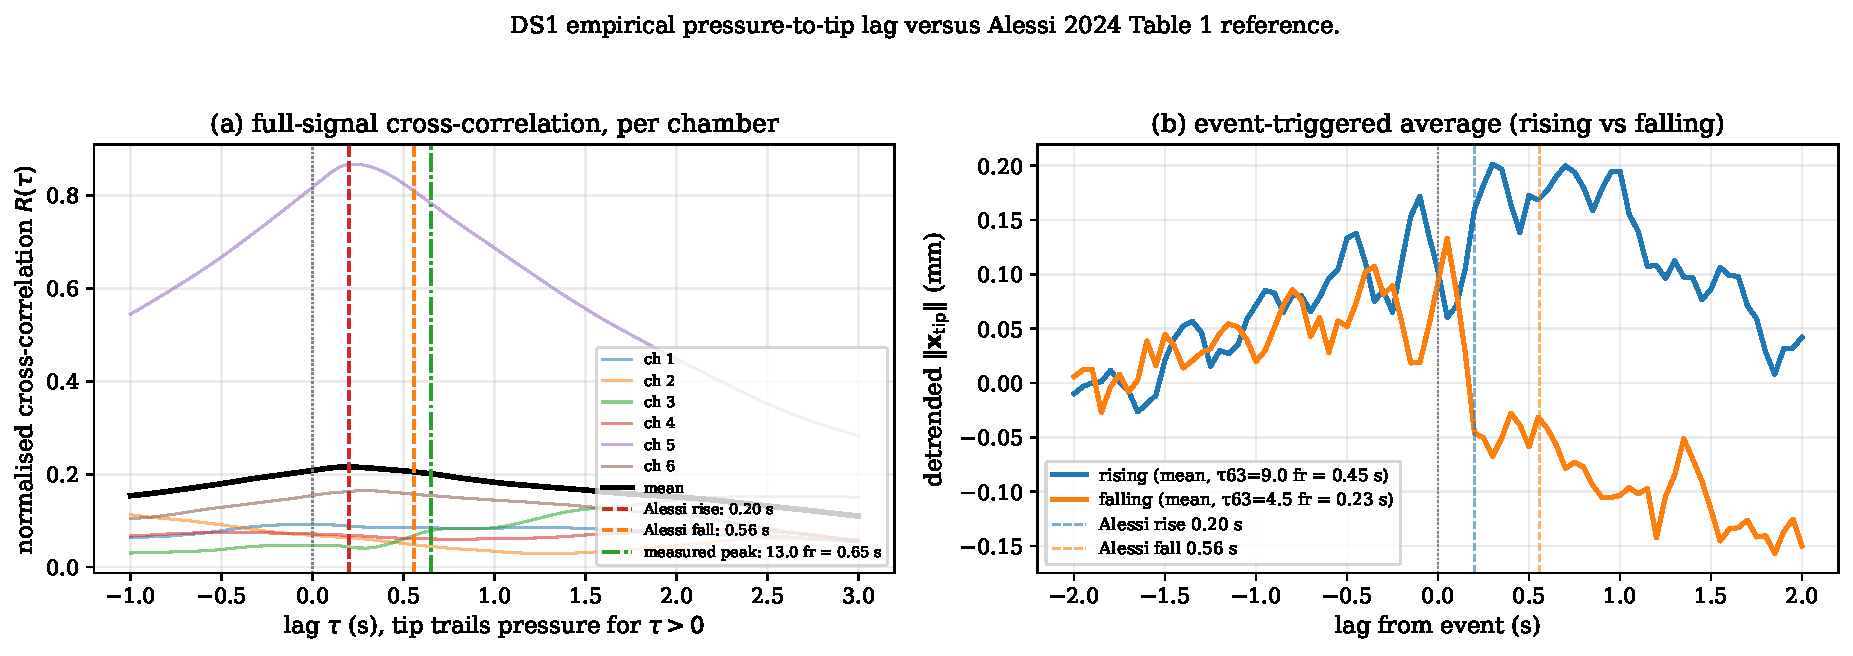
\includegraphics[width=0.98\linewidth]{fig/ds1_pressure_tip_lag.pdf}
  \caption[DS1 empirical pressure-to-tip lag against Alessi 2024.]{Empirical pressure-to-tip lag on Dataset~1's training frames (seeds~1 and 2, $N = 7981$) compared with Alessi et al.\ \cite{alessi2024pushing} Table~1. (a) Normalised cross-correlation $R(\tau)$ of each chamber's pressure against the tip-displacement magnitude; chamber~5 peaks at $\tau = 5$ frames ($0.25$\,s) with $R = 0.87$, within one frame of the $0.2$\,s pressurisation time. The median absolute peak lag across all six chambers is $13$ frames. (b) Event-triggered average of the tip-displacement response to dp/dt extrema (rising and falling templates, mean over six chambers); the random-walk excitation does not cleanly isolate Alessi's asymmetric load/unload transients, but the order-of-magnitude lag agreement is sufficient to motivate a recurrent window $K \geq 10$ frames.}
  \label{fig:app_ds1_lag}
\end{figure}

\section{Reproducibility}
\label{app:reproducibility}

Table~\ref{tab:app_repro_env} lists the software and hardware environment in which every experiment of Chapter~\ref{chap:results} was executed. All numbers reported in this thesis were generated on this single workstation with a fixed random seed of $42$ and cuDNN set to deterministic (\texttt{deterministic=True}, \texttt{benchmark=False}); re-running the training scripts in the same environment reproduces the tabulated metrics to within the last displayed digit.

\begin{table}[!htbp]
  \centering
  \small
  \caption{Software and hardware environment used for all experiments.}
  \label{tab:app_repro_env}
  \begin{tabularx}{\linewidth}{@{}l X@{}}
    \toprule
    Component & Value \\
    \midrule
    Operating system        & Ubuntu 24.04.4 LTS (Linux 6.17.0) \\
    CPU                     & Intel Core i7-13650HX (14 cores, 20 threads) \\
    RAM                     & 16\,GB DDR5 \\
    GPU                     & NVIDIA GeForce RTX 4060 Laptop (8\,GB, CUDA 12.6) \\
    Python                  & 3.11 \\
    PyTorch                 & 2.11.0+cu126 \\
    torchvision             & 0.26.0+cu126 \\
    NumPy / Pandas / SciPy  & 2.4.3 / 3.0.2 / 1.17.1 \\
    scikit-learn            & 1.8.0 \\
    matplotlib              & 3.10.8 \\
    PyElastica              & 0.3.3.post2 \\
    Random seed             & $42$ (Python, NumPy, PyTorch CPU and CUDA) \\
    cuDNN flags             & \texttt{deterministic=True}, \texttt{benchmark=False} \\
    Outer repository commit & \texttt{e9a7d5d} (\textit{soft\_robot\_ai}) \\
    \bottomrule
  \end{tabularx}
\end{table}

\paragraph{Checkpoint layout.}
All trained networks are stored under \texttt{checkpoints/\{experiment\}/\{run\_id\}/best.pt}, where \texttt{experiment} is one of \{\texttt{mlp\_ds1\_tip}, \texttt{mlp\_ds1\_tipmid}, \texttt{mlp\_ds2\_tip}, \texttt{lstm\_ds1\_tip}, \texttt{lstm\_ds1\_tipmid}, \texttt{lstm\_ds2\_tip}, \texttt{fk\_ds1}, \texttt{fk\_ds2}, \texttt{sim2real\_A}, \texttt{sim2real\_B}, \texttt{sim2real\_C}\} and \texttt{run\_id} encodes the date and the configuration hash. Each checkpoint file is a single PyTorch dictionary with keys \texttt{model\_state\_dict}, \texttt{optimizer\_state\_dict}, \texttt{config} (the full YAML used for training), \texttt{input\_scaler}, \texttt{output\_scaler}, \texttt{seed}, \texttt{git\_hash}, and \texttt{timestamp}, following the metadata convention of Section~\ref{sec:reproducibility}.

\paragraph{Evaluation determinism.}
Evaluation scripts load the checkpoint, restore both scalers, re-seed all random-number generators, and run a single forward pass over the frozen test split. No test-time augmentation, dropout, or batch-normalisation update is applied. Closed-loop tracking evaluations use the fixed reference trajectories of Section~\ref{sec:traj} and the same FK arbiter checkpoint for every method, so that any differences between methods are attributable to the methods themselves rather than to arbiter variation.

\paragraph{Code availability.}
The training scripts, evaluation pipelines, configuration files, and figure-regeneration scripts are archived in the project repository described in Appendix~\ref{app:code}. The exact commit associated with the numbers reported in Chapter~\ref{chap:results} is \texttt{e9a7d5d} on the \texttt{master} branch; the raw Dataset~1 pickles and the Dataset~2 CSV are held under \texttt{data/raw/} and are not redistributed because of upstream licensing constraints stated in Appendix~\ref{app:code}.
